\appendix
\label{Anhang}
\section{Anhang}

\subsection{Weitere Aktivierungsfunktionen}\label{anhang:weitereaktivierungsfunktionen}

\begin{figure}[h]
    \center
    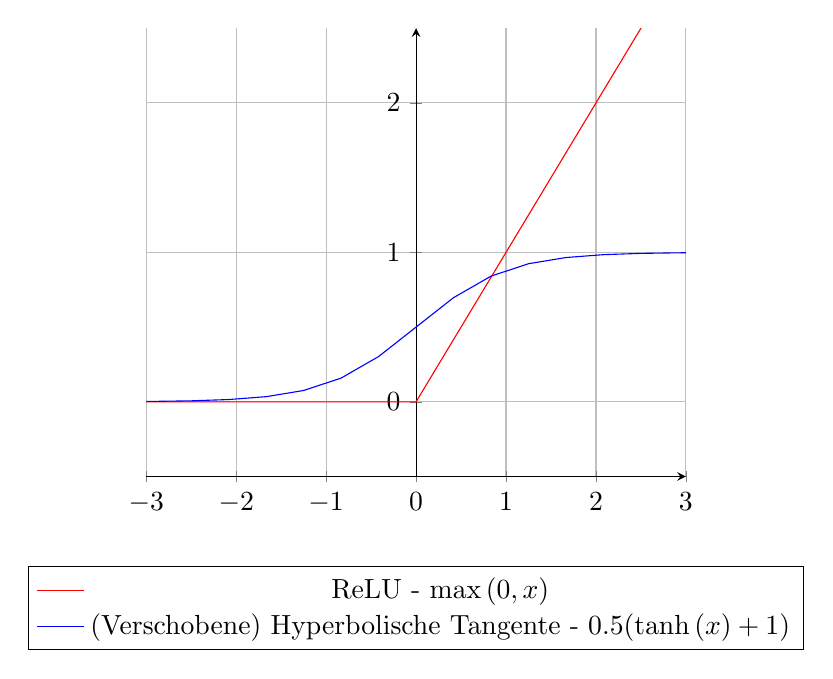
\begin{tikzpicture}
    \begin{axis}
        [
            grid=major,
            xmin=-3,
            xmax=3,
            axis x line=bottom,
            ytick={0,1,2},
            ymax=2.5,
            ymin=-0.5,
            axis y line=middle,
            legend style={at={(0.5,-0.2)},anchor=north}
        ]
        \addplot[red,mark=none]{(x>=0)*x};
        \addplot[blue, mark=none]{0.5*(tanh(\x)+1)};
        \legend{ReLU - $\max{(0,x)}$, (Verschobene) Hyperbolische Tangente - $0.5(\tanh{(x)}+1)$}
    \end{axis}
\end{tikzpicture}
    \caption[Aktivierungsfunktionen]{Weitere Aktivierungsfunktionen, ergänzend zu der Sigmoid Funktion aus Kapitel \ref{funktionsweise}}
    \label{Aktivierungsfunktionen}%
\end{figure}

Die ReLU Funktion (Rectified linear Unit) Funktion ist im Vergleich zu anderen Aktivierungsfunktionen, wie der Sigmoidfunktion oder der Hyperbolischen Tangente, deutlich simpler, was sich in den Leistungsansprüchen des Trainingsprozesses wiederspiegelt.



